 
Adaptive tuning schemes are confronted with two important aspects of tuning. On the one hand, each new chord has to be intoned `vertically', that is, one has to tune the relative pitches between simultaneously played notes. On the other hand, subsequent chords have to be intoned relative to each other in `horizontal' (temporal) direction according to the harmonic progression, as will be discussed in the following section.

\subsection{Vertical tuning at first glance}

In order to tune a given chord vertically, we want to determine the pitches in such a way that the resulting interval sizes are equal or at least close to the ideal ratios of JI. In other words, for a chord consisting of $N$ tones according to the keyboard keys $\{k_1,k_2,\ldots,k_N\}$ we have to find pitches $\{\Lambda_{k_1},\ldots,\Lambda_{k_N}\}$ such that the interval sizes $\Phi_{k_i,k_j}$ agree as much as possible with the values~$\Phi^\JI_{k_i,k_j}$ listed in Table \ref{tablejustint}.

Most of the existing approaches mentioned in the introduction consider only the intervals between \textit{adjacent} tones of a chord. Contrarily the present method also takes intervals between non-adjacent tones into account on equal footing with the others. This means that for a chord consisting of $N$ tones there are $N(N-1)/2$ possible intervals which have to be tuned as just as possible.

As there are $N(N-1)/2$ intervals but only $N$ degrees of freedom, it is clear that it is not always possible to find a consistent solution where all interval sizes $\Phi_{k_i,k_j}$ match exactly with the given cent differences $\Phi^\JI_{k_i,k_j}$. For example, the triad C-E-G can be tuned in just intonation while the triad C-E-G$^\sharp$ cannot.\footnote{C-E-G: Tuning the major third C-E to the ratio 5/4 and the minor third E-G to the ratio 6/5, the resulting fifth C-G has the  ratio $\frac54\cdot \frac65 = \frac32$, meaning that the triad is perfectly consonant in just intonation. Contrarily, for C-E-G$^\sharp$, where two major thirds are combined, the resulting augmented fifth would have the frequency ratio $\bigl( \frac54\bigr)^2=\frac{20}{16}$ which differs from the ratio $\frac85$ listed in the Table \ref{tablejustint}. This means that this chord cannot be tuned consistently in just intonation.} In such a situation, where a chord cannot be tuned consistently in just intonation, the algorithm should render an acceptable tempered compromise. In fact, this is basically what musicians do: they do not solve complicated puzzles of number theory, instead they simply adjust their own pitch on an intuitive basis in such a way that the best possible harmonic compromise is achieved.

The solution investigated in this paper is based on a simple idea which can be explained as follows. As sketched in Fig.~\ref{circuit}, we consider a fictitious battery-resistor network, where each battery has a voltage corresponding to the ideal pitch difference $\Phi^\JI_{k_i,k_j}$ of JI. If the chord can be tuned justly (e.g. as a major triad) the voltages will adjust exactly at the corresponding pitches and the currents passing the resistors are zero. Otherwise, for chords which cannot be tuned justly, the network will produce a certain compromise which depends on the specific choice of the resistors. As already pointed out above, the dissipated power can be regarded as a measure how strongly this tuning compromise is tempered.

\begin{figure}[t]
\fl\begin{minipage}{110mm}
\caption{\label{circuit}Simplified sketch of the vertical tuning scheme suggested in the present paper. The figure shows a keyboard on which a C-Major chord is played. Viewing these keys as electrical contacts we place a battery in series with a resistor between each of the $4\cdot 3/2=6$ possible intervals. Assuming that each battery has a voltage equal to the ideal pitch difference $\Phi^\JI_{k_i,k_j}$ in JI, the resistor network will attain an equilibrium according to Kirchhoff's laws where the voltages at the key contacts represent the desired microtonal pitches. If all electrical currents in the network vanish (as in the present example) the chord is tuned exactly in JI. If not, the specific choice of the resistors determines a tempered compromise where the dissipated power measures how much the chord is tempered. The system is coupled to an external voltage  which controls the reference pitch.} 
\end{minipage}
\vspace{-76mm}
\begin{flushright}
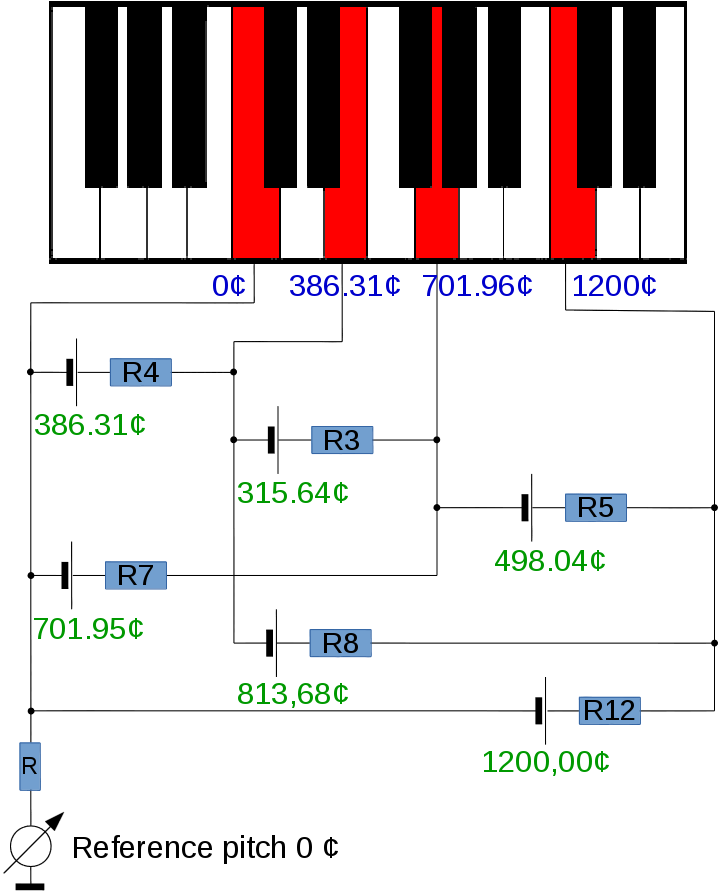
\includegraphics[width=60mm]{circuit} 
\end{flushright}
\end{figure}


\subsection{Mathematical formulation}
Consider a chord of $N$ tones with key indices $k_1,k_2,\ldots,k_N$ in increasing order. The chord consists of $N(N-1)/2$ intervals with index pairs $i,j \in \{k_1,\ldots,k_N\}$ ordered by $i<j$. The task would be to tune the pitches $\Lambda_i$ (with $i\in\{k_1,\ldots,k_N\}$) in such a way that the pitch differences $\Lambda_j-\Lambda_i$  deviate as little as possible from the ideal pitch differences $\Phi^\JI_{k_i,k_j}$ listed in Table \ref{tablejustint}, or equivalently, that the differences $\lambda_j-\lambda_i$ deviate as little as possible from $\phi^\JI_{i,j}:=\phi^\JI_{k_i,k_j}$. We solve this problem by minimizing the squared deviations as follows. Denoting by $\vec\lambda=(\lambda_{k_1},\ldots,\lambda_{k_N})^T$ the vector of pitch deviations from the ET of the pressed keys, we define a deviation potential by
%
\begin{equation}
\label{V1}
V[\vec\lambda] \;=\; \frac14 \sum_{i,j\in \{k_1,\ldots,k_N\} \atop i<j} w_{ij} \Bigl( \lambda_j(t)-\lambda_i(t)-\phi^\JI_{ij}\Bigr)^2 \,,
\end{equation}
%
which is just the sum of all quadratic deviations of the interval sizes weighted by certain factors $w_{ij}$, assuming that $w_{ii}=0$. The weights can be chosen freely and can be viewed as the conductivity of the resistors in Fig.~\ref{circuit}. Their purpose is to determine the `rigidity' of the respective interval in the tuning process. In practice it is meaningful to assign a high weight factor to intervals with simple fractional ratios. In addition, the weight factors may also take the actual volume of the participating tones into account. 

In a more compact notation, the deviation potential (\ref{V1}) can be written in the bilinear form
%
\begin{equation}
\label{GeneralV}
V[\vec\lambda] \;=\; \frac12 \vec\lambda\cdot \mathbf{A} \vec\lambda \;+\; \vec b\cdot \vec\lambda + c\,,
\end{equation}
%
where $\mathbf{A}$ is a symmetric $N\times N$ matrix and $\vec b$ is a vector with the components
%r
\begin{equation}
\label{AB}
A_{ij} \;=\; \left\{
\begin{array}{cc}
-w_{ij} & \mbox{ if } i\neq j  \\
\sum_{\ell} w_{i\ell} & \mbox{ if } i=j 
\end{array}
\right.\,,\qquad
b_i \;=\; \sum_j w_{ij} \,\phi_{ij}
\end{equation}
%
and where
%
\begin{equation}
\label{C}
c=\frac14 \sum_{i,j} w_{ij} \phi_{ij}^2
\end{equation}
%
is a constant. The optimal pitches $\vec\lambda^\OPT$, in which we would like to tune the chord, correspond to a situation where $V[\vec\lambda]$ is minimal, that is $\vec\nabla_\lambda V=\vec 0$, leading to the system of equations $\mathbf{A}\vec\lambda +\vec b=0$. Thus, if $\mathbf{A}$ was invertible, the solution would be given by
%
\begin{equation}
\vec\lambda^\OPT=-\mathbf{A}^{-1}\vec b.
\end{equation}
%
Thus, the whole tuning process amounts to solving a system of linear equations. Finally, the potential 
%
\begin{equation}
\label{eqv}
V[\vec\lambda^\OPT] \;=\; c-\frac12 \vec b \cdot \mathbf{A}^{-1}\vec b
\end{equation}
%
evaluated at $\vec\lambda=\vec\lambda^\OPT$ gives the dissipated power, telling us to what extent the result is tempered.

However, inspecting $\mathbf A$ one can easily see that the column sum is zero, hence the matrix does not have full rank and thus it is not invertible. This can be traced back to the fact that the potential is defined in pitch \textit{differences}, leaving the absolute pitch of the chord undetermined. This can be circumvented easily by coupling the network to an external source which determines the global concert pitch, as described in Appendix~A.

